\section[Background]{Background}
\subsection{Cosmic Expansion}
A spatially homogeneous and isotropic Universe can be described as FLRW metric. Solving Einstein's field equations with FLRW metric gives expansion of the Universe~\cite{TEU}. Hubble parameter $H(t)=\dot{a}(t)/a(t)$ evolves according to~\cite{manual}
\begin{equation}
H^2(t) = H_0^2 \left[ \Omega_\text{rad} a^{-4}(t) + \Omega_\text{mat}a^{-3}(t) + \Omega_\text{curv}a^{-2} (t) + \Omega_\Lambda \right]
\end{equation}

Because of expansion of the Universe, light emitted in the past gets redshifted over time. The redshift of a source is given by~\cite{manual}
\begin{equation}
z=\frac{\lambda_\text{obj}-\lambda_\text{em}}{\lambda_\text{em}}
\label{math:z}
\end{equation}
\noindent
Where, $\lambda_\text{obs}$ and $\lambda_\text{em}$ are, respectively, the wavelengths at time of observation and emission.
Redshift is directly related to the scale factor by~\cite{manual}
\begin{equation}
1+z=\frac{1}{a(t_{em})}
\end{equation}
with scale factor at present time defined as $a(t_0) = 1$. Also, this equation shows that the Universe was half of its current size when a source at redshift $z= 1$ is observed.

The local Hubble law is given by the following formula~\cite{manual}
 \begin{equation}
    v_\text{esc}=H_{0}D
 \label{Hubble}
 \end{equation}
 where $H_{0} = H(t_0)$ is Hubble constant and $D$ is the distance between object and observer.
  
  \subsection{Distances}
  One defines the angular diameter distance in a static Universe as
  \begin{equation}
  	D_\text{ang}(z)=2R/\delta=a(z)f_{K}(w)
  \label{DAngular}
  \end{equation}
  \noindent
  where $R$ is the radius of the distant object, $\delta$ is the angular diameter, and $z$ is the cosmological redshift. If we consider an observer at redshift $ z_{1} $ gives the angular diameter of another object at redshift $ z_{2} $ in FLRW Universe, the equation \ref{DAngular} becomes~\cite{manual}
  \begin{align}
	  \begin{split}
	  D_\text{ang}(z_{1},z_{2}) &=a(z_{2})f_{K}[w(z_{2}) - w(z_{1})] \\
										 &= \frac{1}{1+z_2} f_{K} \left[ \frac{c}{H_0} \int_{z_1}^{z_2} \frac{\dd{z'}}{\sqrt{(1-\Omega_\text{m}-\Omega_\Lambda)(1+z')^2 + \Omega_\text{m}(1+z')^3+\Omega_\Lambda}} \right]					
	  \end{split}
  \label{math:Dangular2}
  \end{align}
  % Another distance measure relates the observed flux, S, of a source to its luminosity, L. For a known luminosity, the distance to the source can be determined as,
  % \begin{equation}
  % D_\text{lum}(z)=\sqrt{\frac{L}{4\pi S}}
  % \end{equation}

\subsection{Quasars}
Quasars (QUASi-stellar radio sources) are an extremely luminous and distant active galactic nuclei (AGN). The power for AGNs comes from accretion of matter onto super-massive black-hole, where the significant fraction of the gravitational energy is released as radiation
% The radiating part of the quasars must be very compact due to the variability nature
%. High variability is also strongly correlated with other three properties: high degree of polarization, compact radio structure and strong $ \gamma $ -ray emission
\cite{manual}. Quasars have variable luminosity which can be used to determine the time delay between lens images.

\subsection{Gravitational lensing}
A gravitational field is caused by distribution of the matter like, a cluster of galaxies between distant light source and an observer. Due to the effects of this field, light rays are bending traveling from a source to an observer. This effect is called the \textit{gravitational lensing}. The general situation of gravitational lensing is considered as in figure.\ref{Fig:lensing}. Here we suppose the mass distribution at distance $ \text{D}_{\text{d}}$, a source is located at distance $ \text{D}_{\text{s}} $, and $ \text{D}_{\text{ds}}$ is the distance from deflector to a source. All distances used in gravitational lensing are the angular diameter distances.
\begin{figure}[H]
	\centering
	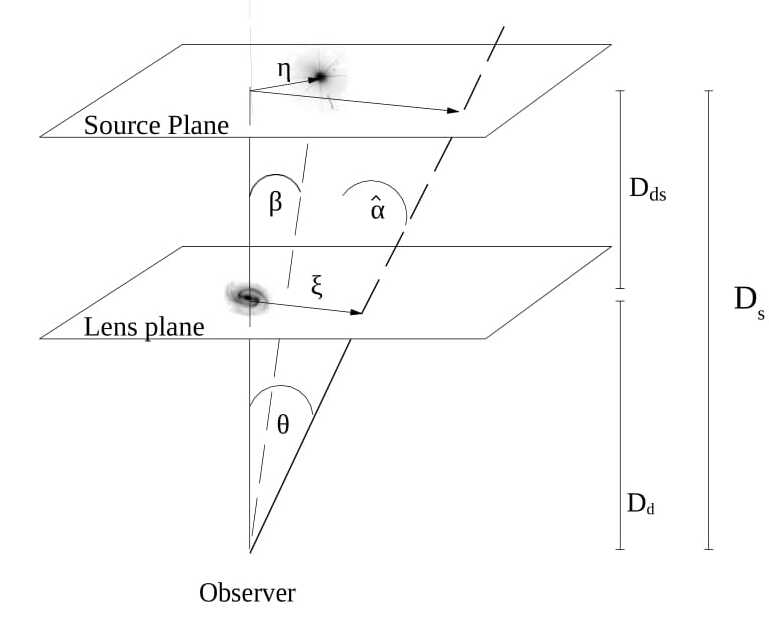
\includegraphics[width=0.6\linewidth]{lensing.jpg}
	\caption{schematic diagram of a gravitational lensing \cite{manual}.}%
	\label{Fig:lensing}
\end{figure}

\subsubsection{Lens Equation}
To study the deflection of light by the lens system, we need some approximations. First, the distance from an observer to lens and lens to a source is very large so that all angles can be considered small i.e. $\tan x \approx \sin x \approx x$. Secondly, source plane and lens plane are parallel, and deflection of light only occur in lens plane as in Born approximation.

For a given source, the lens equation is given by,
\begin{equation}
\pmb\beta =\pmb\theta - \pmb\alpha (\pmb\theta)
\label{LEquation}
\end{equation}
\noindent
where $\pmb\theta$ is the apparent angular position of the source in the sky, $\pmb\beta$ is its true position, and $\pmb\alpha $ is the scaled deflection angle.
% The angles can relates to physical distances as,
% \begin{equation}
% \pmb\eta=\frac{\text{D}_{\text{s}}}{\text{D}_{\text{d}}} \pmb\xi - \text{ D}_{\text{ds}}\hat{\pmb\alpha}(\pmb\xi)
% \end{equation}
% where $\text{D}_{\text{d}}\pmb\theta =\pmb\xi $, $\pmb\eta= \text{D}_{\text{s}}\pmb\beta $, and $ \hat{\pmb\alpha(\pmb\xi)} $ is the true deflection angle.
The scaled deflection angle and true deflection angle are connected with~\cite{manual}
\begin{equation}
\pmb\alpha(\pmb\theta)=\frac{{D}_{\text{ds}}}{{D}_{\text{s}}} \hat{\pmb\alpha}(D_{d}\pmb\theta)
\end{equation}

Convergence is defined as
\begin{equation}
\kappa(\pmb\theta)=\frac{\sum(D_{d} \pmb \theta)}{\sum_\text{cr}}
\label{Equ:KTheta}
\end{equation}
with the critical surface mass density~\cite{manual}
\begin{equation}
\Sigma_\text{cr}=\frac{c^2}{4\pi G}\frac{D_{s}}{D_{d}D_{ds}}
\label{SumCr}
\end{equation}

The scaled deflection angle can be written purely in terms of observable angles~\cite{manual}
\begin{equation}
\pmb\alpha(\pmb\theta)=\frac{1}{\pi}\int \dd[2]{\theta'} \kappa(\pmb{\theta}')\frac{\pmb\theta-\pmb\theta'}{| \pmb\theta -\pmb\theta'| ^2}
\label{ScaledDA}
\end{equation} 
For further convenience, the deflection potential is introduced~\cite{manual}
\begin{equation}
\psi(\pmb\theta)=\frac{1}{\pi}\int \dd[2]{\theta'} \kappa(\pmb\theta') \ln | \pmb\theta- \pmb\theta'| 
\label{psiTheta}
\end{equation}

The use of this quantity is well-motivated because it encloses all information of the mass distribution of the lens~\cite{manual}. In addition, relation of deflection potential and deflection angle can be found
\begin{equation}
\pmb\alpha(\pmb\theta)=\pmb\nabla\psi(\pmb\theta)
\label{Equ:AlphaTheta}
\end{equation}
From the deflection potential a further scalar function, the Fermat potential, can be defined~\cite{manual}
\begin{equation}
\tau(\pmb\theta; \pmb\beta)=\frac{1}{2}(\pmb\beta -\pmb\theta)^2 -\psi(\pmb\theta)
\label{Equ:Format}
\end{equation}

Finally to find the magnification of the images is given by~\cite{manual}
\begin{equation}
\mu =(\det A)^{-1}
\label{math:mag}
\end{equation}
where \text{A} is the Jacobian matrix of lens mapping
\begin{equation}
A_{ij}=\frac{\partial\beta_{i}}{\partial \theta_{j}}
\end{equation}\\

% \subsubsection{Strong lensing}
% Multiple images of a source can be obtain in strong lensing. It can be  describe by considering the Format potential $\tau(\pmb\beta;\pmb\theta) $ with fixing $\beta$ and assuming det$ A \ne 0$~\cite{manual}.
%
% \begin{itemize}
	% \item Minima: det$ A\textgreater 0$, tr $A\textgreater 0$
	% \item Maxima: det$ A\textgreater 0$, tr $A\textless 0$
	% \item Saddle points: det $A\textless 0$
% \end{itemize}
% \noindent
% \textbf{Critical curves and Caustics}: Those points in image plane where the magnification diverges i.e. det $A=0  $ called critical curves. Also, the mapping of a critical curve into the source plane is called caustics. In general, critical curves are closed and smooth. Caustics are closed, but not necessarily smooth.

\subsubsection{The Odd Number Theorem}
If a source has a large offset from line of sight from observer to the lens, it is easy to see only one image. The odd number theorem tells us, when we started with one image there will always be an odd number of images of gravitational lensing; however, normally at least one of them is highly de-magnified. So we can only observe even number of images (mostly double or quadruple images)~\cite{manual}.

\subsubsection{The SIS (Singular Isothermal Sphere)}
A simple model to describe the mass distribution of a galaxy acting as a lens is the singular isothermal sphere (SIS):
\begin{equation}
\rho(r)=\frac{\sigma_{v}^{2}}{2\pi G r^2}
\label{equ:SIS}
\end{equation}
where $ \sigma_{v} $ is the velocity dispersion. Physically this means that the lens system consists of self-gravitating with Maxwellian velocity distribution~\cite{Schneider}.

Integration along the line of sight yields the surface mass density
\begin{equation}
\Sigma(\xi)=\frac{\sigma^2_{v}}{2G\xi}
\label{equ:Sigma(xi)}
\end{equation}

\noindent
A characteristic angular scale of an axisymmetric lens is given by the Einstein radius $ \theta_{E} $ , defined as the angle inside which the mean of the convergence is unity. As a consequence, the projected mass inside $ \theta_{E} $ can be written as~\cite{manual},
\begin{equation}
M(\theta \le \theta_{E})=\pi \theta^2_{E}D^2_{d}\Sigma_{cr}
\label{math:projMass}
\end{equation}
\noindent
We use it to determine the mass of the lensing galaxy. For an SIS the Einstein radius can be calculated as~\cite{manual},
\begin{equation}
\theta_{E}=4\pi\bigg( \frac{\sigma_{v}}{c}\bigg)^2\frac{D_{ds}}{D_{s}}
\label{Equ:ThetaE}
\end{equation}

\subsection{Time Delay}
We have described about multiple images on the topic strong lensing. Light rays of different images have different paths from source to observer, thus there can be different travel times. There are two different contributions of time delay. First one is geometric time delay 
% which comes from the bending of light ray caused by gravity
and second is the potential time delay which induced by the way of light through a gravitational potential~\cite{manual}.

We will find the time delay by using the following expression~\cite{manual}
\begin{equation}
c\Delta t(\beta)=(1+z_{\text{d}})\frac{{D}_{{d}}{D}_{{s}}}{{D}_{{ds}}}[\tau(\pmb\theta_{\text{A}}; \pmb\beta)-\tau(\pmb\theta_{\text{B}}; \pmb\beta)]
\label{Equ:TimeDelay}
\end{equation}
\noindent
Equation \ref{Equ:TimeDelay} shows that the time delay is inverse proportional to the Hubble constant, i.e.
\begin{equation}
\pmb\Delta t \propto \frac{1}{\text{H}_{0}}
\end{equation}

% \begin{figure}[H]
	% \centering
	% 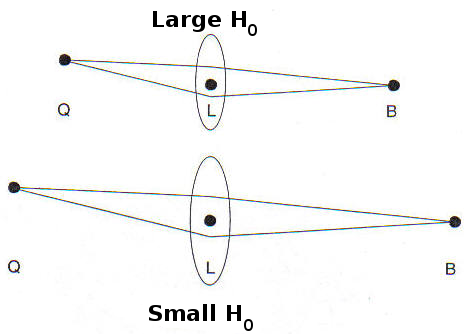
\includegraphics[width=0.6\linewidth]{Ho.png}
	% \caption{Sketch of gravitational lensing system with quasar(Q), lens (L), and observer (B) in two universe with different Hubble constants. The redshift, image position, and flux ration are same for both cases \cite{manual}.}%
	% \label{Fig:H_{0}}
% \end{figure}
% \noindent
% From Fig. \ref{Fig:H_{0}}, it is clearly seen that if we take same redshift, image position, and flux ratio for both cases but there is large difference on the lensing system due to the time delay. Also, it is clear that the time delay and Hubble constant are inversely proportional each other.  \\

In this report, we can use \textit{minimum dispersion method} to calculate time-delays. The light curve for one quasar image is denoted as $ A(t_{k}) $ and other one is $ B(t_{k}) $ which is shifted by time shift $ \lambda $. In this case, the dispersion function $ \text{D}^2 $ is defined as~\cite{manual},
\begin{equation}
\text{D}^2(\lambda, \Delta m)=\sum_{k=1}^{N}(\text{A}(t_{k}) - \text{B}(t_{k}+\lambda, \Delta m) )^2
\label{math:disp}
\end{equation}
where the light curves are sampled at a discrete number of times $ t_{k}$ and $\Delta m$ is the magnitude shift. This method basically search for minimal dispersion in $2$d-plane of $\lambda$ and $\Delta m$.
The error bars of the time delay can be estimated using a Monte-Carlo strategy.

\subsection{Calibration frames}
In astronomical observation, the different kind of calibration frames are necessary for image reduction. These frames are described as following.

\subsubsection{BIAS}
An empty CCD (Charge Coupled Detector) has still get positive numbers due to DC offset that is added in the electronics and A/D converter. In addition there is read out noise present. This is called bias~\cite{manual}. 
% To obtain bias corrected image we have to subtract median BIAS from the image.
A BIAS frame is obtained by taking exposure of no exposure time with shutter closed and the image read out of unexposed CCD. 
% The median bias frame should be made as the median of  10 or more bias frame.

\subsubsection{DARK}
The main purpose of dark frame is to measure the dark current (thermal noise). The dark frames are made by taking expose time equal to the largest exposure time of science frame with shutter closed~\cite{manual}. 
% We have to subtract the median dark frame from the image to obtain corrected image.

\subsubsection{FLAT}
All the pixels of CCD have different quantum efficiency (QE), so they need to be properly normalized. One way to obtain a flat field frame is by illuminating the telescope dome from the inside and taking short exposures as not to saturate the CCD. It is called dome flats and they can always obtain even during daytime. Another way is by sky flats which are obtained by taking exposures during evening and/or morning twilight~\cite{manual}. 
% To make master co-added flat-field image we have to take ten or more flats then averaged together.

\subsection{Image reduction}\label{subsec:imageReduction}
The image reduction is done to remove instrumental signature and improve the signal-to-noise (S/N) in the data before extracting any scientific information\cite{manual}.
\subsubsection{Super-flat and Fringing}
If the flat frame unable to flatten the pixels properly then we should use super-flat. The position of the telescope is slightly displaced every time, dithering, to avoid the same region of the sky falling on to the pixels. It also correct the falling of important data on bad pixels in the image. Science exposures should be used for a super-flat frame~\cite{manual}.
% however, we used dome or twilight for normal flat field frame.

If the variations in the science frame are multiplicative, then the science frame  have to be divided by the supper-flat. However, if the variation are additive, then  we get a fringe pattern which is subtract by de-fringing model. These fringes mainly occur on a CCD image from monochromatic light due to interference. Since fringing is an additive effect so it must be subtracted from the science frame. Fringe model is obtained by smoothing the super-flat with large number of pixels and subtracted from the science images to obtain fully corrected images for pixel-to-pixel variations~\cite{manual}.

\subsubsection{Masking and Weighting }
During the analysis of data, bad pixels cause problems that lead incorrect result. It can be assigning these pixels by a certain value. Then these values recognised by the software programs and neglect them. 
% There are to types of making. First, globing masking, where a mask file is applied to all frames. Second is individual masking which mask the individual pixel.
The mask file contain information about the exposure time which turns them into weight image~\cite{manual}. 
% The weight images are co-added.
\subsubsection{Astrometric Calibration}
The mapping between image co-ordinate and sky co-ordinate. It should done with the help of catalog, so we use reference catalog on-line (SDSS-R9). Then the astrometric solution is calculated by using Scamp software package~\cite{manual}.
\subsubsection{Sky Subtraction}
Along with the target object CCD also collects light from background sky. This has to be removed from the image to get only the flux from the object of interest. To do so, first, we have to remove all the objects in the frame and image has to be smoothed with a specific kernel width. The background image is subtracted from the original frames~\cite{manual}.
\subsubsection{Co-adding}
Stacking all science frame in to one master frame is called Co-adding. One needs to make sure that each objects should fall onto the same pixel. This leads to the high S/N values than individual frames~\cite{manual}.
\subsubsection{Photometric Calibration}
The earth atmosphere play an important role in our observations. Different telescopes have different flux values for the same target in different atmospheric conditions. For standard stars, the relation between instrumental magnitude and true magnitude is given by~\cite{manual},
\begin{equation}
{m}_{\text{calb}}={m}_{\text{instr}}+ {Z}
\end{equation}
where $Z$ is the photometric zero point.
